\section{Introduction}

%Most mobile MR development platforms (i.e. ARCore, and ARKit) utilise a form of \textit{visual odometry} %\cite{yousif2015overview}
%combined with motion or inertial information to map the device's position relative to the real-world, while dedicated HMDs (i.e. HoloLens), leverage multiple cameras with depth sensors to understand the environment and create a virtual 3D map. Once a good mapping has been created, the virtual space (or a coordinate system) is shared with applications to allow synthetic or augmented content to interact with the physical world such as \textit{anchoring} a virtual object on your desk.% This mapping is usually in the form of a 3D \textit{point cloud}.% accompanied by normal vectors to signify orientation of the points which allows for easier surface detection.

% The opening discussion focuses on the necessary processes that delivers the MR services.
AR/MR platforms such as Google ARCore \cite{arcore}, Apple ARKit \cite{arkit}, and Windows Mixed Reality API \cite{windowsMRdev} requires spatial understanding of the user environment in order to deliver virtual augmentations that seemingly inhabit the real world, and, in some immersive examples, even interact with physical objects.\footnote{For the rest of the paper, we will be collectively referring to AR and MR as MR.} The captured spatial information is stored digitally as a spatial map or graph of 3D points, called a point cloud, which is accompanied by mesh information to indicate how the points, when connected, represent surfaces and other structures in the user environment. %Captured visual information are mapped to a digital 3D spatial map with the aid of additional motion and/or depth sensor information. This 3D spatial map is usually stored as a set of 3D points, i.e. $(x, y, z)$, which may be accompanied by additional attributes such as orientation (i.e. normal vectors) or photometric information (e.g. RGB, SIFT feature vector, etc.).  further accompanied by a mesh information that tells which points, when connected, form surfaces.
%However, even with only the 3D point information left -- even without additional attributes -- much of the objects within the space or the space itself can still be identified.
%\textbf{Why 3D?} 

However, despite 3D data being a structural representation of the real world, 3D data is perceptually latent from the users. With images and video, what the ``machine sees'' is what the ``user sees'' and a great deal of privacy work have been done on these data forms. Contrariwise, in MR, the experience is exported as visual data (e.g. objects augmented on the user's view) while the underlying spatial mapping, and its extent, as well as the density of the captured points, is not exposed to the users: what the machine sees is different--arguably, even more--than what the user sees. That is, the digital representation of the physical world is not exposed to the user and that the user is oblivious about the captured spatial mapping data. This inherent perceptual difference creates a latency from user perception and, perhaps, affects--or the lack thereof--how users perceive the sensitivity of 3D information.

Aside from the the spatial structural information, the mapping can also include 3D maps of objects within the space. Furthermore, the spatial map can also reveal the location of the user: the general location as well as the user's location within the space. Similarly, most users are oblivious about the various information that are included in the spatial maps captured and stored by AR/MR platforms.

\begin{figure}[t]
	\centering
	\begin{minipage}[]{\columnwidth}
		\subfloat[1][A generic information flow (following the green solid arrows) for a desired MR functionality $G$ with an attacker $J$ which can perform adversarial inference off line to determine the space the user is in as well as the objects within the space: (1) adversarial inference \textit{modeling} or \textit{learning} from, say, historical 3D data, and (2) adversarial inference or \textit{matching} over currently released 3D data]{%
			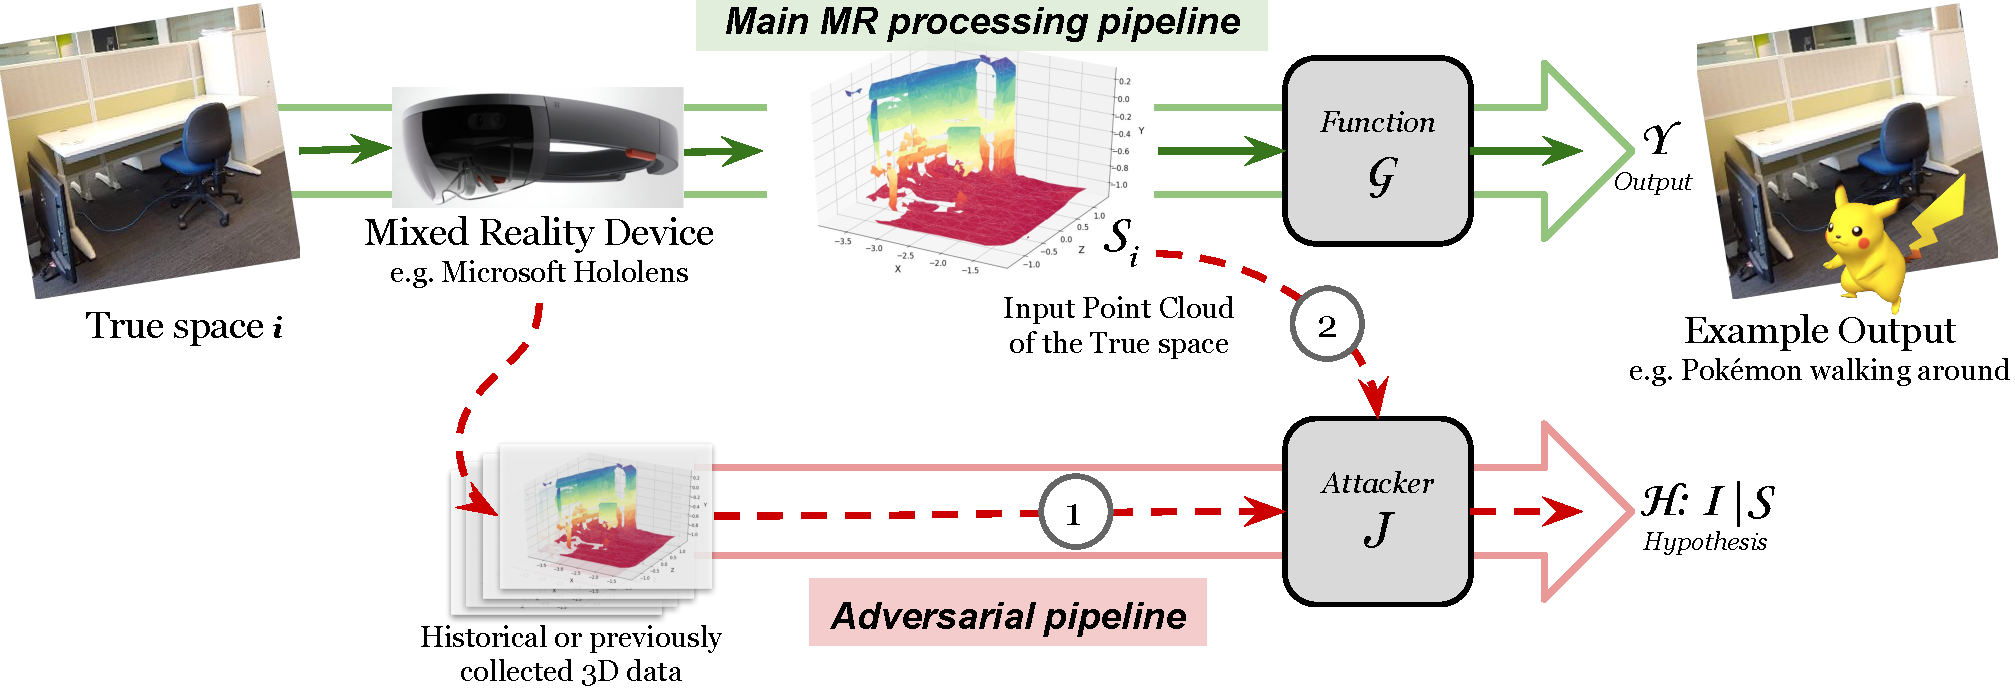
\includegraphics[width=\textwidth]{figures/adversary-model-pipeline-v6-revised-a.pdf}
			\label{fig:generic-pipeline}
			\vspace{5mm}
		}
	\end{minipage}
	\begin{minipage}[]{\columnwidth}
		\subfloat[2][Inserting an intermediate privacy-preserving mechanism $M$ which aims to prevent spatial inference]{%
			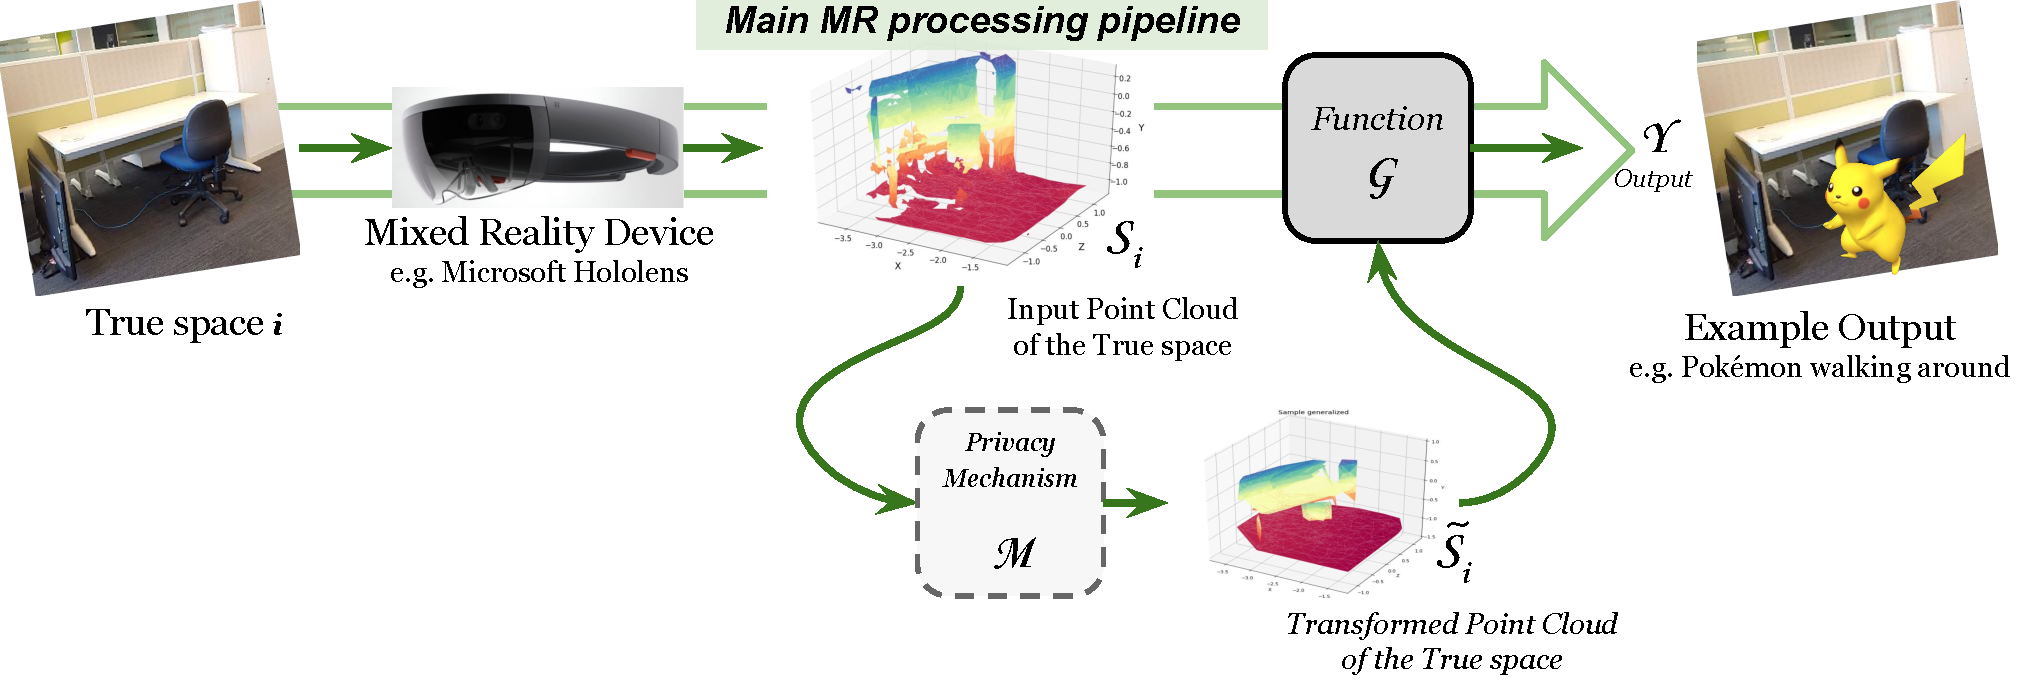
\includegraphics[width=\textwidth]{figures/adversary-model-pipeline-v6-revised-b.pdf}
			%\caption{}
			\label{fig:with-privacy-mechanism}
		}
	\end{minipage}
	%\makebox[0pt]{
	%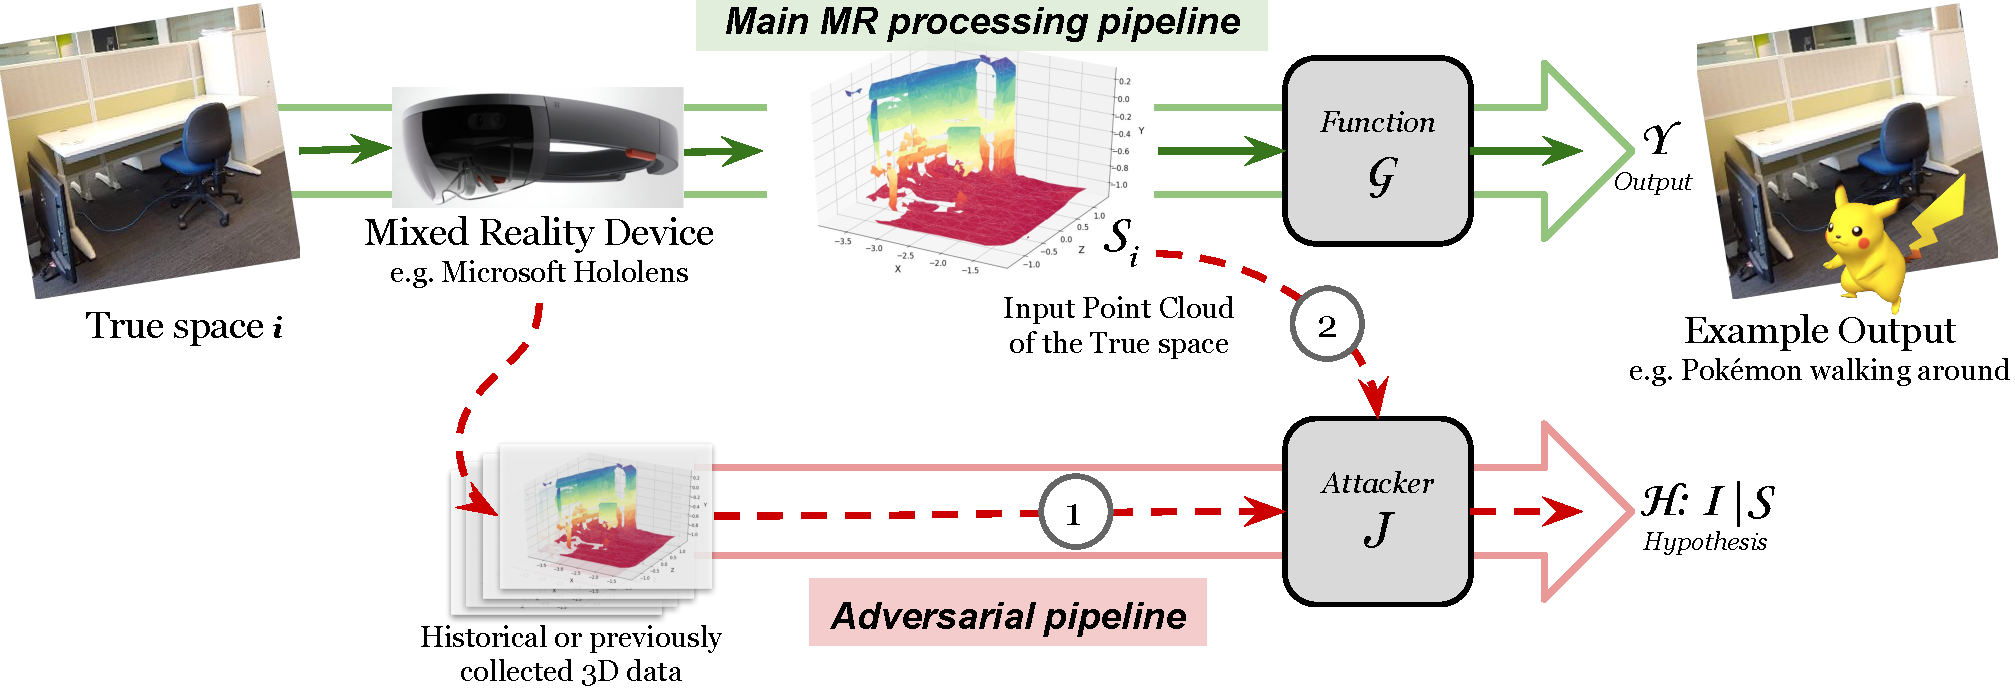
\includegraphics[width=\columnwidth]{figures/adversary-model-pipeline-v6-revised-a.pdf}%,height=0.12\textheight}
	%\vspace{-2mm}
	\caption{\small AR/MR pipeline diagrams with (a) an attacker, and (b) an introduced intermediary privacy mechanism.}
	\vspace{-4mm}
	\label{fig:adversary-model-pipeline}
\end{figure}

Fig. \ref{fig:generic-pipeline} presents a generic process or information flow diagram for an MR service. The device captures the spatial information of the space and stores it as a 3D point cloud which can be provided to applications to deliver their intended functions, say, augmenting a virtual monster on the floor. However, these 3D spatial maps that may contain sensitive information which the user did not intend to expose can be stored and, then, accessed by a potential adversary (also shown in Fig.\ref{fig:generic-pipeline}) and be further utilized for functionalities beyond the application's intended function such as aggressive localized advertisements. And, so far, there are no mechanisms in place that ensure user data privacy in MR platforms.

As majority of the work on MR have been focused on delivering the technology, %\cite{grubert2017pervasiveAR}
only recently have there been efforts in addressing the security, safety, and privacy risks associated with MR technology. There have been a few older works which have pointed out the non-technical issues such as ethical considerations \cite{heimo2014ethical}, and value-sensitive design approaches \cite{friedman2000value} that highlights the need to consider data ownership, privacy, secrecy, and integrity in MR. Moreover, a recent study has focused on the potential perceptual and sensory threats that can arise from MR outputs such as photosensitive epilepsy and motion-induced blindness \cite{baldassi2018challenges}. In conjunction to these expositions, the EU have recently legislated the General Data Protection Regulation (GDPR) which aims to address privacy issues from a policy approach. It aims to empower the users and protect their data privacy. This further highlights the importance of designing and developing \textit{privacy-enhancing technologies} (PETs) especially those that can be applied to the MR use case.

Our earlier work \cite{deguzman2019firstlook} provided preliminary evidence of how easy it is for an adversary to infer spaces from captured 3D data. And how, even with spatial generalization (i.e. the 3D space is generalized in to a set of planes), spatial inference is still possible at a significant success rate. In this work, we extend our previous work with an improved attacker that not only identifies the space but also infers the user's location within the space. To construct the attacker, we build up on existing place recognition methods that have been applied on 3D lidar data and modify it to be usable for the scale on which 3D data is captured by MR platforms. Then, we present spatial generalizations with conservative releasing as a privacy approach. %We also utilize an extended dataset that includes various indoor and outdoor scenes.

%Most of the work on MR for the past two decades has focused on delivering the necessary technology to make MR a possibility. As the necessary technology matures, MR devices, like any other technology, will become more available and affordable. Consequently, the proliferation of these devices may entail security and privacy implications which may yet not be known. For example, it has been demonstrated how facial images captured by a web camera can be cross-matched with publicly available online social network (OSN) profile photos to match the names with the faces and determine social security numbers \cite{acquisti2011}. %\cite{wang2015visually}
%With most MR devices coming out in a wearable, i.e. head-mounted, form-factor and having at least one camera to capture the environment, it will be easy to perform such facial matching tasks in the wild without the subjects knowing it. Security and privacy in these systems, more often than not, comes as an afterthought, as shown in this survey paper.

%The recent EU-GDPR ruling aims to address these issues from a policy approach. It aims to empower the users and protect their data privacy. This highlights the importance of designing and developing \textit{privacy-enhancing technologies} (PETs). %While the GDPR can be considered as the most important change in data privacy regulation,
%Currently, there are numerous PETs designed for structured data such as \textit{k}-anonymity\cite{sweeney2002k}, and \textit{differential privacy}\cite{dwork2014algorithmic}, as well as techniques for data aggregation during information collection\cite{he2011pda}. However, current techniques protecting media are mostly for conventional data types, and are primarily focusing on \textit{facial de-identification} for \textit{identity privacy} \cite{newton2005preserving,  gross2008semisupervised, wu2018privacy, brkic2017generative,  gross2006model, du2014garp,} as well as protection against visual capture recording mechanisms\cite{acquisti2011, zarepour2016context}. (See \cite{deguzman2018security} for a survey of MR-related security and privacy protection approaches.)%acquisti2011, zarepour2016context,

%Quickly on related work: Despite having numerous current related work on 3D object deteciton, this is the first work that focuses on spatial privacy and how generalization can still be leveraged in preserving privacy.

%Furthermore, current MR platforms (i.e. Windows MR, ARCore and ARKit) directly operates on these 3D spatial maps or point clouds and, so far, no privacy preservation is applied before providing these data to third party applications.

%Describe the privacy problem using the Fig.\ref{fig:adversary-model-pipeline} ..

%In this work, we focus on the \textit{nascent risks} %from captured and collected 3D data used for MR processing. To demonstrate the privacy leakage, we utilize actual 3D point cloud data, captured by a Microsoft HoloLens, to construct an adversarial inferrer that can identify spaces from the revealed 3D data. The inference performance is evaluated over both raw data and different 3D data generalizations. And we show how such generalizations are ineffective even with a simple \textit{matching-based} inference attack. To the best of our knowledge, this is the first work that aims to expose these risks. Consequently, we make the following specific contributions in this work:

To the best of our knowledge, we are the first to expose spatial privacy risks on 3D spatial data captured by MR platforms. We have demonstrated how easy it is to extend the scope of 3D recognition algorithms to be used as an attacker in the MR scenario. To this end, we summarize the major contributions of this work as follows:

\begin{enumerate}%[leftmargin=*]
	\item First, we formalize the \textit{3D spatial privacy problem} and define the privacy and utility metrics specific to 3D MR data.
	\item We present an \textit{3D adversarial inference model} that reveals the general space of a user, i.e. inter-space inference, and their specific location within the space, i.e. intra-space inference or, commonly, tracking attack.%, e.g. point sampling factor by 3.
	%In particular, we define the 3D adversarial inference using the well-established Bayesian inference as basis.
	\item Using 3D point cloud data collected from Microsoft HoloLens, which is also the same 3D data representation format for Google's ARCore and Apple's ARKit, we demonstrate that 3D spatial inference attacks are possible on these MR platforms.
	\item We demonstrate that the insufficient protection provided by spatial generalizations can be improved by conservatively releasing the generalizations; specifically, we control the release of plane generalizations rather than giving out the generalizations entirely. %However, %as well as the 	negative impact on utility of these generalizations. 
	\item We also show that we can get better data utility with a smaller size of space while providing adequate privacy. 
	\item Lastly, we present an in depth analysis over a realistic scenario when user spaces are successively released and experimentally determine the minimum number of releases, and planes that prevents spatial inference, both inter-space and intra-space.
	%\item Lastly, we 
	%delaying release of small partial spaces (with radius $r<0.25$) and maintaining a low number of planes, i.e. $< 5$, can delay inference and potentially provide privacy. %in conjunction with a localized generalization.
	%higher number of planes can be inferred more precisely but does not necessarily improve recall or reduce error rate.
	%\item Lastly, we show the \textit{memory compactness} of 3D data which emphasizes how adversaries can create lightweight 3D inference models of user spaces.
\end{enumerate}

%RETURN HERE AFTER REARRANGING ALL THE SECTIONS.

The rest of the paper is organized follows. First, we discuss the related work in \S\ref{sec:related-work}. Then, \S\ref{sec:framework} presents the theoretical framework of spatial privacy problem and the definitions of the elements of the framework as well as the adversary model. In \S\ref{sec:privacy-preservation}, we describe the various information reduction techniques we can employ to prevent spatial inference. Likewise, we describe in \S\ref{sec:3d-space} the different description and inference methods an adversary may utilize for spatial inference. We present the evaluation methodology in \S\ref{sec:methodology} to investigate the viability of privacy methods we employ over varying experimental setups. The results are presented in \S\ref{sec:results} followed by the discussion in \S\ref{sec:discussion}. We conclude the paper in \S\ref{sec:conclusion}. % and \S\ref{sec:future_work}, respectively. 

\section{Related Work}\label{sec:related-work}

In the general privacy and security space, various work have already been done--from revealing privacy leakage in online social networks \cite{krishnamurthy2010privacy} and mobile devices \cite{ren2016recon}, to developing privacy-preserving mechanisms for conventional user data types \cite{sweeney2002k, mcsherry2007mechanism, dwork2014algorithmic} as well as against deep-learning inference \cite{shokri2015privacy, abadi2016deep}. From Sections \ref{rrw:vision} to \ref{rrw:others} we focus on the various privacy-related work in MR, and present in \ref{rrw:3d-methods} the existing 3D recognition methods available which can be utilized as the basis of a 3D spatial attacker.

\subsection{Traditional approaches to visual data protection}\label{rrw:vision}
%Most of the earlier privacy protection techniques for MR were primarily focused on \textit{visual} information or media (i.e. image and video) sanitization \cite{jana2013scanner,raval2014markit, roesner2014world, aditya2016pic, raval2016you, shu2016cardea, li2016privacycamera, zarepour2016context}. Aside from that are \textit{abstraction} approaches to privacy protection. In the specific 3D use case, significant work have been done on protections involving abstracting physiological information \cite{jana2013scanner, figueiredo2016prepose} using the idea of \textit{least privilege} \cite{vilk2014least}. The same approach has also been used for providing visual privacy when using 3D MR browsers \cite{vilk2015surroundweb};  when actual walls and surfaces are utilized as displays, the 3D browsing applications displayed through them need not know where these surfaces are in the real physical environment; however, it did not specifically protect against spatial inference. A very recent work also utilized the idea of least privilege to apply visual abstractions for mobile MR \cite{deguzman2019safeMR}.

There are several MR and related \textit{privacy-enhancing techniques} (PETs) that have been proposed in the literature as listed in \cite{deguzman2018security}. Early approaches primarily involved applying sanitization techniques on visual media. %To maintain and control the utility of information, 

\subsubsection{Sanitization techniques} The \textsc{Darkly} system inserts an intermediary input protection layer to implement \textit{multiple level} feature sanitization for specific objects which allows users to control the amount of detail or features which can be provided to applications \cite{jana2013scanner}. %, i.e. stricter policies means less features are provided.
Context-based sanitization has also been applied by detecting pre-defined sensitive objects or contexts (e.g. in toilet) in the captured images, and automatically implements sanitization by blurring or outright deletion \cite{zarepour2016context}. Another recent work focused on a more tangible solution which cuts off capturing of a head-worn camera by physically covering it when sensitive contexts are detected \cite{steilPrivaceye2018}. However, these systems only focuses primarily on protecting objects or data that are \textit{explicitly} included on predefined policies which can be myopic, and blinded from external and \textit{latent} sensitive information.

Extrinsic input protection approaches arise from the need for permission from sensitive objects external to the user that are not considered by the intrinsic policies. In fact, there are a good number of work on environment-driven input protection enforcement. For example, \textit{world-driven} access control was proposed to allow non-users to specify their privacy preferences through a shared database \cite{roesner2014world}. Similarly, \textsc{I-pic} allows users to endorse their privacy choices through Bluetooth Low Energy (BLE) and sanitize captured images accordingly \cite{aditya2016pic}. Other similar works are \textsc{PrivacyCamera} that uses cooperation to blur other visually captured users using their endorsed GPS and privacy choice information \cite{li2016privacycamera}, and \textsc{Cardea} that uses gestures to endorse user privacy choices \cite{shu2016cardea}. All these previous works on externally-driven input protection relies on a form of database or communication channel, e.g. BLE, that is shared among users. The shared database can exclude users or objects that are not part of the database which still defeats the purpose of an environment-driven input sanitization.

Most of the extrinsic sanitization techniques discussed so far are focused on the face as the sensitive object in trying to address \textit{bystander} privacy. Although, it is important to protect \textit{bystander} privacy, object protection is necessary for universal protection. \textsc{MarkIt} uses privacy markers, i.e. visual indicators, and gestures to endorse sensitive objects or texts to capture devices \cite{raval2014markit}. It was integrated to Android's camera subsystem to prevent applications from leaking private visual information \cite{raval2016you}. \textsc{MarkIt} is a step closer to selective object protection, but it requires markers for detection of sensitive objects. Also, it does not provide protection for the latently sensitive objects.

However, all these sanitization approaches, are all focused on post-captured images which can still pose security and privacy risks. Moreover, these approaches have only been applied on the wide use case of visual capture devices and not on the specific mixed reality use case.

%Live and on-the-fly sanitization has also been demonstrated by performing fast face recognition and video sanitization \cite{wang2017scalable}. 

\subsubsection{Abstraction-as-Protection} Abstraction approaches addresses the earlier issues with sanitization by reducing or eliminating the necessity of accessing the raw visual feed directly. %primarily on visual media or information.
The \textsc{Recognizers} approach inserts a hierarchical recognizer to provide input sanitization and input access control over the hierarchical recognized data \cite{jana2013enabling}. Another work builds up on the this work and focuses on the implementation of privilege separation \cite{thompson2016securing}. Similar principles of abstraction and \textit{least privilege} access were also applied to secure rendering for 3D browsers \cite{vilk2014least,vilk2015surroundweb}. %Specifically, in 3D browsing, actual walls and surfaces are utilised as displays, and the browsing applications displayed through them need not know where these surfaces are in the real physical environment. 
Another abstraction-based PET focuses on user gesture detection for using gestures as user inputs. \textsc{Prepose} only sends the gesture events to the applications which effectively removes the necessity to have access to the raw (i.e. RGB and depth camera) input feed \cite{figueiredo2016prepose}. On the output-side, similar intermediary abstractions can be inserted before the renderer to ensure secure and safe rendering \cite{lebeck2016safely}, e.g. prevent malicious or misleading augmentations. The same approach has also been used for providing visual privacy when using 3D MR browsers \cite{vilk2015surroundweb};  when actual walls and surfaces are utilized as displays, the 3D browsing applications displayed through them need not know where these surfaces are in the real physical environment but it did not specifically protect against spatial inference. A very recent work also utilized the idea of least privilege to apply visual abstractions for mobile MR \cite{deguzman2019safeMR}. %However, a \textit{trusted} platform, where the abstractions are usually implemented, has to ensure, maintain, and control utility of the information released to untrusted third party applications and services.

However, most of these abstraction-as-protection approaches are targeted over specific input types such as physiometric information (i.e. faces, user gestures, and so on), and have not specifically provided protection against spatial recognition attacks.
%/or have not been implemented and evaluated on a mobile device, i.e. a handheld MR device such as a smartphone. %If not, then, a necessary reputation-based core has to be in place to ensure reliability of abstractions, whether in the input- or output-side.

%\subsection{Other Protection Areas and Strategies}
%%CAN BE REMOVED??
%\textit{Other Protection Areas and Strategies.} Other work focused on how to enable secure data transmission using MR devices which are note necessarily aimed at protecting visual information, such as \textsc{LooksGoodToMe} authentication which leverages on wireless localization to cross-authenticate users using MR head-mounted devices (HMD) \cite{gaebel2016looks}. Another recent work, \textsc{HoloPair} avoids the use of wireless localization, which may be unavailable (and inefficient) to most current devices, and instead utilizes exchange of visual cues between users to confirm the shared secret \cite{sluganovic2017holopair}.
%Other areas of protection focused on how to enable secure data transmission using MR devices. \textsc{LooksGoodToMe} authentication is leveraged on the camera and wireless capabilities of MR head-mounted devices (HMD) \cite{gaebel2016looks}. It uses facial recognition combined with wireless localization information to cross-authenticate users. \textsc{HoloPair}, on the other hand, avoids the use of wireless localization, which may be unavailable (and inefficient) to most current devices, and instead utilizes exchange of visual cues between users to confirm the shared secret \cite{sluganovic2017holopair}. Another recent work utilised secret sharing and secure multi-party computation \cite{sekhavat2017privacy} to provide virtual cloth try-on renders of users using combined sensitive anthropometric user information and public cloth measurement information. PrivacEye \cite{steilPrivaceye2018} is another recent work which also addresses visual privacy but involves a physical form of protection by mechanically closing the ``eye"-view of a first person camera.

\subsection{3D data on MR: attacks, risks, and protection approaches}\label{rrw:3d}
A few recent work have started to look into and expose the actual risks brought about by unprotected and indefinite access to 3D data by MR applications. Using machine learning, original scenes can be revealed from structure from motion (SfM) 3D point cloud data with additional sparse SIFT or other photometric information \cite{pittaluga2019revealing}. A concurrent work focused on presenting a privacy-preserving method of pose estimation to counter these risks. It removes the necessity for 3D point cloud data by instead using 3D line cloud--effectively obfuscating 3D structural, i.e. geometrical, information--during pose estimation \cite{speciale2019privacy}; however, the 3D line cloud approach only addresses the pose estimation functionality and does not present the viability of its usability for surface or object detection which is necessary for a virtual object to be rendered or ``anchored'' onto. Thus, it would still be necessary for 3D point cloud data to be exposed but, perhaps, with some privacy-preserving transformations to hide sensitive content and further prevent spatial recognition. %Furthermore, even with the absence of additional photometric information, spatial location of 3D point cloud data can still be recognized given that adversaries have access to an ensemble of historical 3D point cloud data \cite{deguzman2019firstlook}. 

\subsection{Other protection approaches}\label{rrw:others}
Other recent works have focused on protecting MR outputs specifically in ensuring user safety \cite{lebeck2016safely, lebeck2017securing}. Furthermore, as MR devices allow for new modes of \textit{collaboration}, issues on \textit{power imbalance} brought by the \textit{directionality} of MR interfaces \cite{benford1996shared, benford1998boundaries} are now being studied as well \cite{lebeck2018towards}. %A more extensive collection of security and privacy approaches targeting MR are listed and discussed in \cite{deguzman2018security}.


\section{Conclusion}\label{sec:conclusion}
Currently, MR services are provided full and indefinite access to the 3D spatial information, i.e. 3D point cloud data, captured by an MR-capable device. In this work, we highlight that the risks associated to the indefinite access of applications to these 3D point cloud data. Our preliminary work have presented preliminary evidence of these risks \cite{deguzman2019firstlook}. We have earlier demonstrated how a descriptor-based inferrer can be used for 3D spatial inference. Using this inferrer, we can identify, i.e. inter-space inference, the current space of the MR user using the 3D point cloud information provided by the MR device to the MR service. We enhance this inter-space inferrer in this work.

Furthermore, we have extended the capability of the inferrer to also reveal the exact location within the space, i.e. instra-space inference, of the user. Our validation results reveal that, unsurprisingly, raw 3D point cloud data readily reveals the specific location of spaces with average intra-space error of as low as $1 m$. And that naive spatial generalizations, i.e. using the RANSAC plane-fitting algorithm, is still inadequate.%cannot protect against this kind of inference.

Therefore, it is necessary to provide users with a form of protection, i.e. privacy preserving 3D point cloud releasing. %This was the primary goal of this work.
This time, we have demonstrated that we can enhance the protection from plane generalizations by simply conservatively releasing the generalized planes provided to applications. Our emulated experimental investigation reveals that we can reveal upto 13 planes and avoid inter-space inference half the time. Specifically, with such very conservative releases, the success rate of an (inter-space) inferrer is no better than a random guess. And, for the occasions that the adversary correctly recognizes the space, the intra-space location can be off by at least 3 meters. Moreover, we have shown a quantification of how much we can improve both $\Pi_1$ and $\Pi_2$ by reducing the size of the partial spaces to be revealed. Consequently, in terms of data utility $Q$, a smaller size is anyway preferred to provide good (i.e. low) $Q$. %Similarly, for intra-space inference, for those correctly ``guessed'' spaces will be off by 5 meters or farther.

Overall, these results provides quantities, i.e. thresholds, that allows us to potentially protect users and their spaces as they user MR services. Moreover, we have only utilized simple approaches to spatial privacy protection. Generalization are already implemented in most MR platforms. Thus, what remains is the implementation of conservative plane releasing to provide protection.
%For future work, a practical investigation can provide us with the impact of our presented simple approach on usability of the MR application provided with such generalizations. Furthermore, we also plan to investigate the effectiveness and impact of adding plane perturbations, i.e. translation and/or rotation. %Future work, 1) perturbations, i.e. plane translation and/or rotation; 2) practically demonstrate a proof-of-concept using at least an HMD and a mobile device, then, measure QoE. A practical investigation can provide us with actual user feedback on whether our approach affects the usability of the application or not.
